\chapter{Arquitetura analítica multivisão}\label{arquitetura-analuxedtica-multivisuxe3o}

A arquitetura atual evita a concentração de todos os sinais em um único escore caixa-preta. Cada família produz uma evidência com semântica própria, organizando o fluxo em quatro camadas sequenciais: (i) extração de qualidade e contexto cadastral ($S_{comm}$ e vínculo vigente), com filtragem de séries elegíveis; (ii) detecção de mudança de regime ($t^*$) e cálculo paralelo dos especialistas comportamental ($S_{behavior}$), elétrico ($S_{elec}$) e de eventos físicos ($S_{tamper}$); (iii) aplicação de regras físicas determinísticas e corroboração espacial por alimentador; e (iv) ordenação e triagem operacional.

\section{\texorpdfstring{Especialista de comunicação - \(S_{comm}\)}{Especialista de comunicação - S\_\{comm\}}}\label{especialista-de-comunicauxe7uxe3o---s_comm}

O objetivo de \(S_{comm}\) é responder se a telemetria possui integridade suficiente e se o próprio comportamento de comunicação é atípico. Os atributos considerados incluem cobertura, quantidade de gaps, maior gap, concentração noturna de faltantes e latência de eventos.

Essa separação é essencial porque missingness pode ser informativa para comunicação e, ao mesmo tempo, contaminante para uma inferência física. O gating de qualidade deve ser parametrizável. Um valor como 70\% de cobertura em 30 dias pode ser utilizado inicialmente como hipótese de engenharia, mas não deve ser apresentado como limiar validado antes da análise de sensibilidade.

\section{Change Point Engine}\label{change-point-engine}

O bloco de mudança de regime produz atributos como:

\begin{itemize}
\item
  instante estimado da mudança \(t^*\);
\item
  magnitude relativa \(\Delta\mu\);
\item
  direção da mudança;
\item
  persistência do novo patamar;
\item
  tempo desde a mudança;
\item
  alteração da dispersão antes e depois do evento.
\end{itemize}

Esses atributos acrescentam informação que estatísticas agregadas de janelas fixas não capturam adequadamente.

\section{\texorpdfstring{Especialista elétrico - \(S_{elec}\)}{Especialista elétrico - S\_\{elec\}}}\label{especialista-eluxe9trico---s_elec}

O especialista elétrico utiliza atributos de consumo, corrente, tensão e comportamento temporal. A arquitetura privilegia modelos cuja função possa ser explicada, como Isolation Forest para isolamento multivariado ou PCA residual para erro de reconstrução.

O objetivo não é somar arbitrariamente diversos detectores. Cada escore precisa responder uma pergunta e possuir um plano de validação.

\section{\texorpdfstring{Especialista comportamental - \(S_{behavior}\)}{Especialista comportamental - S\_\{behavior\}}}\label{especialista-comportamental---s_behavior}

O comportamento diário é tratado como uma camada intermediária entre as medições intervalares e as janelas históricas longas. O objetivo é responder não apenas \textbf{quanto} uma UC consumiu, mas \textbf{como} esse consumo se distribuiu ao longo do dia e com que recorrência esse formato aparece.

A representação começa com dias de cobertura adequada. Cada curva é decomposta em duas componentes: magnitude diária e forma normalizada. Essa separação permite que dois consumidores de escalas distintas sejam reconhecidos como semelhantes quanto à rotina intradiária, sem eliminar a informação de consumo total.

Após regularização da cadência, as curvas normalizadas podem ser reduzidas por PCA \autocite{jolliffe2002} e agrupadas com K-Means \autocite{macqueen1967} ou método equivalente \autocite{geron2025}. Os centroides não recebem significado causal automaticamente; são inicialmente \textbf{arquétipos matemáticos de dia}. A interpretação posterior pode identificar, por exemplo, perfis predominantemente diurnos, noturnos, constantes ou bimodais.

\begin{figure}
\centering
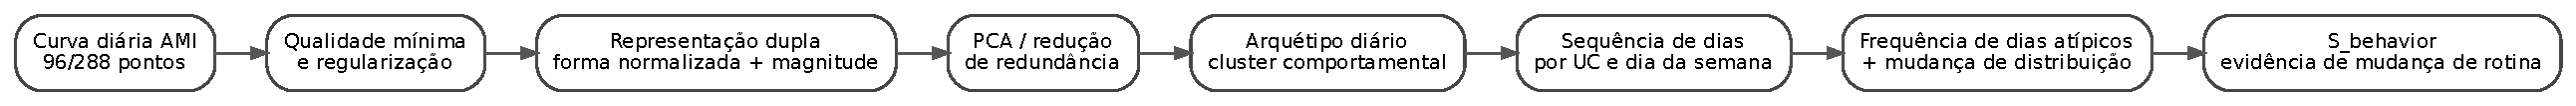
\includegraphics[width=0.94\textwidth,height=0.65\textheight,keepaspectratio]{figures/behavior.pdf}
\caption{Fluxo proposto para o especialista comportamental diário.}\label{fig:behavior}
\par\small Fonte: elaboração própria.
\end{figure}

O diagrama comportamental distingue uma observação de um dia, o arquétipo atribuído à sua forma e a sequência desses arquétipos ao longo do tempo. A passagem de um cluster a outro é uma descrição de mudança de padrão; sua interpretação exige contexto de calendário, qualidade da série e persistência. Clusterização, isoladamente, não atribui causa.

\subsection{Recorrência e dias atípicos}\label{recorruxeancia-e-dias-atuxedpicos}

Um dia diferente não é, por si só, uma anomalia operacional. Uma UC pode apresentar sistematicamente um sábado distinto dos dias úteis. O modelo deve aprender a recorrência condicional ao calendário.

Defina \(c_{u,d}\) como o arquétipo atribuído ao dia \(d\) da UC \(u\). Para cada dia da semana \(w\), pode-se estimar a distribuição histórica

\[q^{base}_{u,w}(c)=P(c_{u,d}=c\mid weekday(d)=w).\]

Um dia recebe escore de atipicidade quando seu perfil tem baixa compatibilidade com a distribuição histórica correspondente. A proporção de dias atípicos em uma janela \(W\) é dada pela Equação \eqref{dias}:

\begin{equation}\label{dias}
R_A(u,W)=\frac{\sum_{d\in V_{u,W}}A_{u,d}}{|V_{u,W}|},\qquad |V_{u,W}|>0,
\end{equation}

\noindent onde $V_{u,W}$ é o conjunto de dias válidos da UC na janela, e $A_{u,d}=1$ para dia comportamentalmente atípico e zero caso contrário. Sem dias válidos, a taxa é indisponível. Trata-se de uma representação de recorrência, e não de um escore calibrado do agrupador.

O sinal de interesse não é apenas \(R_A\) elevado, mas sua mudança:

\[\Delta R_A=R_A(u,W_{recent})-R_A(u,W_{base}).\]

Também pode ser monitorada a mudança da distribuição de arquétipos entre janelas, por exemplo por divergência de Jensen--Shannon \autocite{lin1991}. Dessa forma, uma rotina semanal estável pode permanecer normal mesmo contendo dias diferentes, enquanto o aparecimento de novos tipos de dia ou o aumento persistente de sua frequência gera evidência de mudança comportamental.

\subsection{Interpretação operacional}\label{interpretauxe7uxe3o-operacional}

\(S_{behavior}\) não deve diagnosticar férias, troca de morador, veículo elétrico, geração ou fraude. A sequência de classes permite investigar se a rotina intradiária mudou de forma persistente; não constitui um escore de risco calibrado. A explicação é buscada em cadastro, troca de titularidade, GD, topologia, alarmes e demais especialistas.

Essa camada complementa o CPD (baseado em detecção sequencial de mudanças de nível, como CUSUM \autocite{page1954} e métodos *offline* \autocite{truong2020}). O CPD identifica mudanças de nível ou distribuição ao longo do tempo; \(S_{behavior}\) identifica mudanças na composição dos tipos de dia, inclusive quando a energia diária total permanece aproximadamente constante.

\subsection{Especialistas por alimentador}\label{especialistas-por-alimentador}

Os arquétipos poderão ser treinados globalmente e comparados com modelos locais por alimentador. A hipótese é que alimentadores com composição de carga distinta produzam espaços comportamentais também distintos. O uso de especialista local só será mantido quando houver amostra suficiente e ganho mensurável sobre o modelo global; caso contrário, utiliza-se a referência global ou uma coorte agregada.

\section{\texorpdfstring{Especialista de eventos físicos - \(S_{tamper}\)}{Especialista de eventos físicos - S\_\{tamper\}}}\label{especialista-de-eventos-fuxedsicos---s_tamper}

Alarmes de tampa, campo magnético, falha de fase, alteração de relógio e troca de medidor são tratados como evidências contextuais. Eles não devem, isoladamente, constituir target de fraude. Seu valor aumenta quando coincidem temporalmente com mudança de regime ou anomalia elétrica.

\section{Corroboração espacial e topológica}\label{corroborauxe7uxe3o-espacial-e-topoluxf3gica}

Uma alteração individual ganha significado diferente de uma alteração compartilhada por várias UCs do mesmo transformador ou alimentador. A comparação por alimentador oferece contexto para investigar fenômenos locais e coletivos. A falta de vínculo confiável a transformadores limita a análise sistemática nesse nível.

\section{Formalização da pontuação, fusão e roteamento}\label{formalizauxe7uxe3o-da-pontuauxe7uxe3o-fusuxe3o-e-roteamento}

A expressão ``fusão dos especialistas'\,' descreve \textbf{operações diferentes} no software, que precisam ser separadas para reprodução: consenso entre detectores estatísticos elétricos, regras diagnósticas entre visões e combinação hierárquica entre modelos treinados em diferentes populações. Misturar esses três níveis em uma única expressão \(S=\sum w_m S_m\) faria parecer que há um modelo unificado calibrado para fraude, o que não corresponde ao código disponível.

\subsection{Primeiro nível: consenso dos detectores elétricos}\label{primeiro-nuxedvel-consenso-dos-detectores-eluxe9tricos}

Duas versões do detector elétrico foram desenvolvidas ao longo do projeto. A configuração preliminar do comitê combinava \textbf{quatro detectores} (Isolation Forest, LOF, ECOD e PCA residual), com normalização min--max na própria coorte e bônus de regra física. Essa variante explica a evolução do sistema e os ensaios didáticos iniciais, \textbf{não devendo ser confundida com o ensemble OOT reportado em novembro}.

Na campanha \texttt{OOT\_MULTIVIEW} de 19/11/2026, o especialista elétrico emprega \textbf{seis detectores}: Isolation Forest (IF), LOF, ECOD, COPOD, HBOS e PCA residual. Para a observação \(i\) e o detector \(m\), define-se \(s_{i,m}\) como o escore bruto orientado para que valores maiores indiquem maior raridade. A normalização utiliza os limites dos quantis $P_{01}$ e $P_{99}$ congelados no conjunto de ajuste:

\[z_{i,m}=\operatorname{clip}_{[0,1]}\!\left(\frac{s_{i,m}-a_m}{b_m-a_m}\right),\qquad a_m=Q_{0,01}^{train}(s_m),\quad b_m=Q_{0,99}^{train}(s_m).\]

Quando \(b_m-a_m<10^{-12}\) (amplitude degenerada por empates em cauda), adota-se o quantil superior estendido ($P_{99,9}$) ou os extremos de treino com compressão logarítmica para evitar o esmagamento dos escores. O escore elétrico combinado é definido por:

\[S_{elec,i}^{(6)}=\operatorname{clip}_{[0,1]}\!\left(\sum_{m\in\{\mathrm{IF},\mathrm{LOF},\mathrm{ECOD},\mathrm{COPOD},\mathrm{HBOS},\mathrm{PCA}\}}w_mz_{i,m}+0{,}15R_i\right),\]

com pesos \(\mathbf w=(0{,}22;0{,}20;0{,}18;0{,}18;0{,}10;0{,}12)\) e \(R_i\in\{0,1\}\) representando a ativação da regra elétrica crítica da política. Os pesos e o bônus são escolhas heurísticas de projeto, não estimativas de parâmetros de um modelo supervisionado. Sua sensibilidade individual é avaliada nos ensaios de ablação. O bônus de \(0{,}15\) não é peso de detector. As regras permanecem condições de triagem e não confirmação de violação regulatória ou fraude.

A validação temporal definiu o limiar de referência \(\tau_{train}=0{,}5131\) na execução consolidada pós-saneamento (\texttt{20261125\_134559\_972\_oot\_multiview}), obtido exclusivamente no conjunto de ajuste anterior ao corte. A seleção deve ser lida conjuntamente com qualidade, regras diagnósticas e política operacional; logo, \(S_{elec,i}\ge\tau_{train}\) isoladamente não é sinônimo de candidato final. Esse limiar permanece congelado na avaliação fora do tempo.

A configuração preliminar de quatro detectores pode ser escrita, para comparação, como:

\[S_{elec,i}^{(4)}=\operatorname{clip}_{[0,1]}\!\left(0{,}30z_{i,IF}+0{,}25z_{i,LOF}+0{,}25z_{i,ECOD}+0{,}20z_{i,PCA}+0{,}20R_i\right).\]

Essa expressão representa uma configuração anterior, com normalização e corte dependentes do lote; não é utilizada para justificar quantitativos do experimento OOT de seis detectores. A ablação do ensemble é reportada à parte, comparando Top-K em coorte fixa. O registro da configuração, artefatos de treino, normalização e política é condição de reprodução do escore.

\subsection{Segundo nível: gate de confiabilidade e diagnóstico multivisão}\label{segundo-nuxedvel-gate-de-confiabilidade-e-diagnuxf3stico-multivisuxe3o}

O \texttt{ElectricalAnomalyDetector} calcula o escore elétrico e marca sua confiabilidade por:

\[G_i=\mathbb{I}(q_i\ge g),\qquad g=0{,}70\ \text{na configuração padrão da plataforma},\]

em que \(q_i\) é o indicador de qualidade disponibilizado ao módulo. A condição elétrica positiva utiliza \(D_iG_i\), com \(D_i=\mathbb{I}(S_{elec,i}\ge\tau)\) e \(\tau\) definido pela versão do detector e da política de decisão. O \textbf{escore bruto continua disponível} na saída do modelo mesmo quando \(G_i=0\); o gate restringe a declaração de anomalia elétrica, sem suprimir o cálculo numérico do escore. No orquestrador hierárquico, o indicador booleano de elegibilidade para ajuste (\emph{clean-for-train}) seleciona amostras limpas e encaminha séries degradadas para quarentena, com \emph{fallback} quando há poucas observações válidas. Assim, existem controles de qualidade em \textbf{estágios distintos} do fluxo que não devem ser confundidos.

O módulo de comunicação utiliza Isolation Forest e ECOD, combinando os dois escores normalizados como:

\[S_{comm,i}=0{,}5z_{i,IF}^{comm}+0{,}5z_{i,ECOD}^{comm}.\]

O especialista de eventos físicos aplica saturação da contagem de alarmes \(a_i\), penalidade da inclinação temporal negativa \(b_i\) (em \(\mathrm{kWh/dia^2}\), normalizada pela escala empírica de \(5\ \mathrm{kWh/dia^2}\)) e contexto de substituição \(m_i\in\{0,1\}\):

\[S_{tamper,i}=\operatorname{clip}_{[0,1]}\!\left[0{,}70\min(a_i/3,1)+0{,}30\operatorname{clip}_{[0,1]}\!\left(-\frac{b_i}{5\ \mathrm{kWh/dia^2}}\right)+0{,}15\mathbb{I}(a_i>0)m_i\right].\]

Os valores dos pesos e da escala de \(5\ \mathrm{kWh/dia^2}\) são heurísticos de projeto, não coeficientes estimados de uma distribuição de irregularidades confirmadas. O agrupador comportamental ajusta PCA e K-Means e retorna \textbf{rótulos de cluster}. Portanto, nessa implementação, não existe um \(S_{behavior}\) probabilístico único que possa ser diretamente somado às demais visões. A recorrência de dias atípicos amplia a interpretação comportamental como representação temporal e não deve ser descrita como escore final já calibrado sem uma função e validação próprias.

A integração multivisão constrói um \textbf{vetor de diagnóstico}:

\[\mathbf e_i=(S_{comm,i},S_{elec,i},S_{tamper,i},G_i,\kappa_i,R_i),\]

em que \(\kappa_i\) é o identificador do cluster comportamental. Em seguida aplica uma árvore de regras com precedência explícita. Na versão inicial de triagem, a sequência de regras priorizava: (1) \(S_{tamper,i}\ge0{,}70\); (2) não confiável com \(S_{comm,i}\ge0{,}70\); (3) não confiável; (4) confiável com \(S_{elec,i}\ge0{,}70\); (5) comunicação anômala; (6) demais casos. Algumas \emph{strings} legadas usam palavras como \texttt{CONFIRMADA} ou \texttt{OPERACAO\_REGULAR}; neste trabalho, elas são tratadas como \textbf{códigos internos de roteamento}, jamais como confirmação de fraude, de ausência de irregularidade ou de conformidade regulatória.

Essa árvore \textbf{não produz um escore contínuo global único} para todas as visões. Caso a carteira necessite de uma prioridade escalar posterior, deve-se especificar versão da função operacional, critérios de elegibilidade, tratamento de valores ausentes, calibração dos escores e estratégia de desempate. A definição dessa política de fila não pode ser retroativamente atribuída ao orquestrador multivisão como se já fosse parte de seu treinamento.

\subsection{Terceiro nível: MoE global versus alimentador}\label{terceiro-nuxedvel-moe-global-versus-alimentador}

No módulo de roteamento hierárquico, a combinação entre escalas é distinta da fusão entre \(S_{comm}\) e \(S_{elec}\). O módulo ajusta um detector composto global e detectores compostos por alimentador para coortes com pelo menos 30 registros, calculando pesos de referência de acordo com o tamanho do alimentador:

\begin{longtable}[]{@{}
  >{\raggedright\arraybackslash}p{(\columnwidth - 6\tabcolsep) * \real{0.2500}}
  >{\raggedleft\arraybackslash}p{(\columnwidth - 6\tabcolsep) * \real{0.2500}}
  >{\raggedleft\arraybackslash}p{(\columnwidth - 6\tabcolsep) * \real{0.2500}}
  >{\raggedleft\arraybackslash}p{(\columnwidth - 6\tabcolsep) * \real{0.2500}}@{}}
\caption{Pesos nominais do roteamento hierárquico}\label{tab:integracao4}\\
\toprule\noalign{}
\begin{minipage}[b]{\linewidth}\raggedright
Registros no alimentador \(n_f\)
\end{minipage} & \begin{minipage}[b]{\linewidth}\raggedleft
\(w_f\)
\end{minipage} & \begin{minipage}[b]{\linewidth}\raggedleft
\(w_r\)
\end{minipage} & \begin{minipage}[b]{\linewidth}\raggedleft
\(w_g\)
\end{minipage} \\
\midrule\noalign{}
\endfirsthead
\toprule\noalign{}
\begin{minipage}[b]{\linewidth}\raggedright
Registros no alimentador \(n_f\)
\end{minipage} & \begin{minipage}[b]{\linewidth}\raggedleft
\(w_f\)
\end{minipage} & \begin{minipage}[b]{\linewidth}\raggedleft
\(w_r\)
\end{minipage} & \begin{minipage}[b]{\linewidth}\raggedleft
\(w_g\)
\end{minipage} \\
\midrule\noalign{}
\endhead
\bottomrule\noalign{}
\endlastfoot
\(n_f<150\) & 0,15 & 0,45 & 0,40 \\
\(150\le n_f<1000\) & interpolação linear de 0,35 a 0,70 & interpolação de 0,40 a 0,20 & interpolação de 0,25 a 0,10 \\
\(n_f\ge1000\) & 0,70 & 0,20 & 0,10 \\
\end{longtable}
{\small\noindent Fonte: elaboração própria.\par}


Aqui \(f\), \(r\) e \(g\) representam alimentador, regional/municipal e global. Havendo penetração de GD no perfil do circuito superior ao limiar configurado, a heurística amplia o peso local, respeitando limites e renormalização. Na variante histórica de treinamento, a chamada de combinação usa escores de \textbf{alimentador e global}, mas passa o escore municipal como \texttt{None}; nesse caso, o operador renormaliza apenas os pesos dos especialistas disponíveis:

\[S^{MoE}_i=\frac{\sum_{m\in\mathcal A_i}w_mS_{i,m}}{\sum_{m\in\mathcal A_i}w_m},\qquad \mathcal A_i\subseteq\{f,r,g\}.\]

Exemplo: com \(n_f\ge1000\) e apenas alimentador/global disponíveis, os pesos nominais \((0{,}70,0{,}20,0{,}10)\) tornam-se efetivamente \(0{,}875\) local e \(0{,}125\) global. O limiar de decisão pode ser obtido por quantis locais sobre registros elegíveis. Isso mostra que o componente ``Mixture of Experts'\,' atualmente implementado é um \textbf{roteador hierárquico heurístico de modelos}, não uma rede neural com \emph{gating network} treinada por gradiente no sentido clássico de \textcite{jacobs1991}. As faixas de 150 e 1.000 registros e os pesos são heurísticas para limitar a influência de coortes pequenas e favorecer referências locais em coortes maiores. A escolha não estabelece suficiência amostral universal e não foi otimizada com desfechos de campo.

\subsection{Propagação das evidências em duas UCs observadas}
No corte de 19/11, a UC 908***00 teve inclinação da energia diária \(b_i=-0{,}4434\)~kWh/dia\(^2\), cobertura de 81,48\% e escore elétrico de 1,0000. A política a encaminhou para investigação de possível GD. A UC 291***96 também apresentou escore elétrico alto (0,8236), mas a cobertura registrada na decisão foi de 3,33\%. A política a encaminhou para análise de comunicação. A Seção~\ref{estudos-caso-reconciliados} confronta essas decisões com os registros físicos e cadastrais.

\subsection{Sensibilidade, estabilidade e critérios de reprodutibilidade}\label{sensibilidade-estabilidade-e-crituxe9rios-de-reprodutibilidade}

Cada configuração é reprodutível apenas quando também se registram: o conjunto usado no \texttt{fit}, os hiperparâmetros, a versão de cada detector, o pré-processamento, o esquema de escores, a coorte de normalização, a política de limiar e as regras físicas executadas. Como o \texttt{fit\_and\_score} multivisão executa ajustes e pontuação no mesmo conjunto passado pelo chamador, sua execução descritiva não constitui, isoladamente, teste de generalização fora da amostra. A avaliação comparativa deve preservar separação temporal e parâmetros treinados congelados.

Os três níveis descrevem operações distintas: consenso elétrico, classificação multivisão por precedência e ponderação hierárquica. Na campanha retrospectiva fora do período de ajuste (\texttt{OOT\_MULTIVIEW}), executou-se o consenso elétrico de seis detectores combinado ao gate de cobertura e às regras diagnósticas de triagem. Os módulos de mudança de regime (CPD), recorrência comportamental, eventos físicos (\(S_{tamper}\)) e roteamento hierárquico por alimentador foram implementados e avaliados separadamente em nível arquitetural e modular, permanecendo a integração simultânea de todos os especialistas em um único escore calibrado como etapa de continuidade. A validação de pesos e limites requer testes de ablação e, para conclusões sobre furto, rótulos externos de inspeção.

\section{Saídas como padrões de compatibilidade}\label{sauxeddas-como-padruxf5es-de-compatibilidade}

A saída analítica evita diagnósticos causais não sustentados. Em vez de emitir ``irregularidade confirmada por evidência independente'', o sistema utiliza classes descritivas de compatibilidade: padrão compatível com redução abrupta de carga, geração local, problema de medição, degradação de telemetria, comportamento estatisticamente atípico ou comportamento corroborado (ou não) pela vizinhança. A qualificação operacional ocorre por cruzamento de evidências --- por exemplo, queda persistente de FA associada a tensão estável, boa cobertura, ausência de mudança coletiva entre pares e alarme físico próximo ao instante $t^*$, elevando a prioridade de análise humana sem substituir a decisão de campo.
